%% SCC26 Purple Team 1 - technical poster (DRAFT SCAFFOLD).
%% Follows poster/README.md (A0 portrait, 3-column, >=40% visual, address-free).
%% Build on Overleaf or a full TeX Live:  pdflatex main.tex  (tikzposter in texlive-full).
%% Figures are reused from ../paper/figures/ ; the Week-5 ones regenerate via
%% project/tools/w5paper.sh, the architecture one from ../paper/figures/architecture.mmd.
%% NO real addresses: logical and Terraform-variable names only (instructor rule).
\documentclass[25pt, a0paper, portrait, margin=0mm, innermargin=14mm,
  blockverticalspace=12mm, colspace=14mm, subcolspace=8mm]{tikzposter}

\usepackage{graphicx}
\usepackage{booktabs}
\usepackage{amsmath}
\graphicspath{{../paper/figures/}}

\usetheme{Default}
\usecolorstyle{Denmark}

\title{Evidence-Driven Security Observability in an\\ OpenStack--Kubernetes Student Cyber Range}
\author{Student A \quad Student B \quad Student C \quad Student D}
\institute{CHPC / NICIS --- SCC26 Student Project, South Africa}

\begin{document}
\maketitle

\block{Research question}{%
  \centering\Large\itshape
  Can a small team make detection, response and an automated incident explanation all
  \textbf{driven by retained evidence}, so that every claim traces to a captured artifact?%
}

\begin{columns}

%% ---------------- COLUMN 1 ----------------
\column{0.34}

\block{1.~Problem \& why it matters}{
  \begin{itemize}
    \item Security telemetry is often added late, hand-configured, and reported with
      numbers that cannot be reproduced.
    \item It is easy to claim a detection that was never really tested, or a response
      time measured against the defender's own, already-understood traffic.
    \item Goal: a cluster where detection, response and incident explanation are
      \textbf{evidence-driven} --- every figure retraces to a captured artifact.
  \end{itemize}
}

\block{2.~Architecture (address-free)}{
  \begin{tikzfigure}
    \IfFileExists{../paper/figures/architecture.pdf}
      {\includegraphics[width=0.95\linewidth]{architecture.pdf}}
      {\framebox[0.9\linewidth]{\rule{0pt}{9cm}renders from architecture.mmd}}
  \end{tikzfigure}
  \begin{itemize}
    \item Five hosts; only \texttt{edge-01} is Internet-facing (WireGuard, Pi-hole DNS,
      nftables, Suricata IDS, Wazuh manager, the one floating IP).
    \item Private Kubernetes net: HAProxy, control plane, two workers; \texttt{kubectl}
      only on the control plane, over the VPN.
    \item Kubernetes~1.36.4 + Cilium~1.20.1, Argo~CD~v3.5.0 GitOps, Traefik~v3.7.14.
    \item All addresses are Terraform variables --- never in the repo or this poster.
  \end{itemize}
}

\block{4.~Evidence sources \& provenance}{
  \begin{itemize}
    \item \textbf{Host:} Wazuh rules (break-glass 100110, rejected/brute 100111/112,
      escalation 100100, single-source correlation 100101).
    \item \textbf{Network:} Suricata SIDs 9000010--9000015 (scan, SSH burst, traversal,
      SQLi, scanner-UA). \textbf{Ops:} Prometheus.
    \item Raw stays on hosts; repo holds only sanitised summaries + a SHA-256 per raw
      file + logical names, validated against schema \texttt{scc26-week5-run/1}.
    \item Tables/figures regenerate from the run directories --- no hand-entered numbers.
  \end{itemize}
}

%% ---------------- COLUMN 2 ----------------
\column{0.32}

\block{3.~Method}{
  \begin{enumerate}
    \item Freeze platform state: pinned commit, Argo \emph{Synced/Healthy}, clocks
      within 1\,s.
    \item Baseline window (10--15\,min, ambient traffic only).
    \item Marked scenario: benign, pre-declared attacker actions from a range host
      against our \emph{own} platform (authorised in \texttt{SELF-RANGE-AUTH.md}).
    \item Export Wazuh + Suricata evidence; merge into one correlated timeline.
    \item Compute $T_\text{detect/identify/contain/recover}$; validate manifest
      (plan + final).
    \item Reset/replay to a clean state between runs.
  \end{enumerate}
}

\block{5.~Key results}{
  \begin{tikzfigure}
    \IfFileExists{../paper/figures/week5/phases.pdf}
      {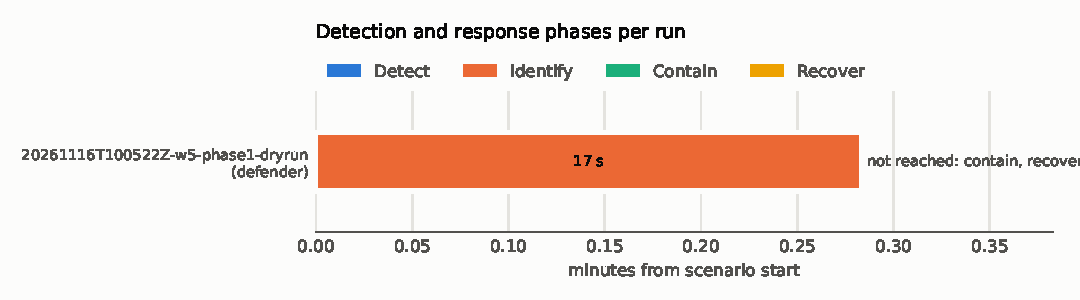
\includegraphics[width=0.96\linewidth]{week5/phases.pdf}}
      {\framebox[0.9\linewidth]{\rule{0pt}{7cm}run project/tools/w5paper.sh}}
  \end{tikzfigure}
  \vspace{4mm}
  \IfFileExists{../paper/figures/week5/metrics.tex}
    {\begin{center}\resizebox{0.98\linewidth}{!}{\begin{tabular}{llrrrrrrrr}
\toprule
Run & Role & T\_detect & T\_identify & T\_contain & T\_recover & Detections & FP & FN & Gaps \\
\midrule
20261116T100522Z-w5-phase1-dryrun & defender & 0 s & 17 s & not reached & not reached & 5 & 2 & 1 & 2 \\
\bottomrule
\end{tabular}
}\end{center}}
    {}
  \begin{itemize}
    \item Every deployed signature fires; host and network evidence correlate on one
      timeline; first detection in \textbf{0--7\,s}.
    \item HTTP run: all four application-layer SIDs, \textbf{zero false negatives}.
    \item Two gaps found and then closed; informational false positives separated.
  \end{itemize}
}

\block{6.~Interpretation \& lessons}{
  \begin{itemize}
    \item The pipeline works end-to-end on the self-range; times are \emph{lower bounds}
      against known, benign, pre-marked traffic.
    \item \textbf{Lesson:} Suricata stamps alerts at \emph{flow-start} (~2--3\,s early),
      so evidence windows must pad $\ge$10\,s or edge detections fall outside the window
      and look like misses.
    \item Negative results (a tooling bug, un-exercised SIDs) are kept and fixed, not
      hidden.
  \end{itemize}
}

%% ---------------- COLUMN 3 ----------------
\column{0.34}

\block{Correlated detection timelines}{
  \begin{tikzfigure}
    \IfFileExists{../paper/figures/week5/timeline-20261116T100522Z-w5-phase1-dryrun.pdf}
      {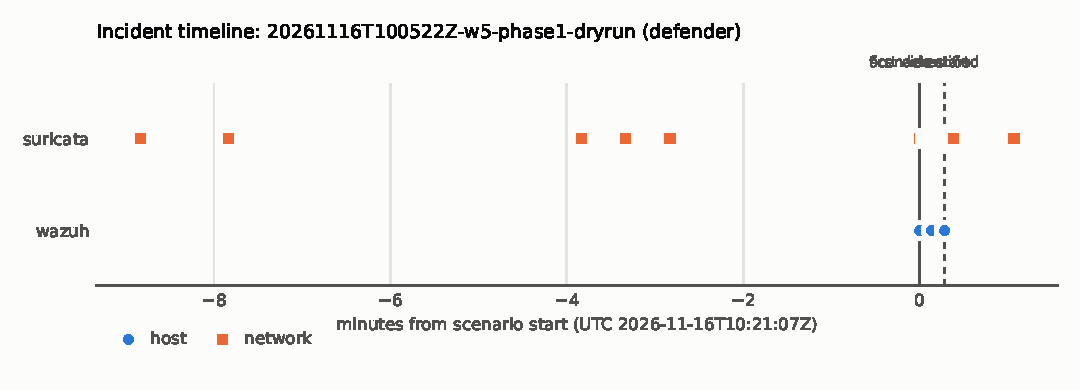
\includegraphics[width=0.98\linewidth]{week5/timeline-20261116T100522Z-w5-phase1-dryrun.pdf}}
      {\framebox[0.9\linewidth]{\rule{0pt}{6cm}timeline (generated)}}
  \end{tikzfigure}
  \vspace{3mm}
  \begin{tikzfigure}
    \IfFileExists{../paper/figures/week5/timeline-20261116T112654Z-w5-phase1-httpsids.pdf}
      {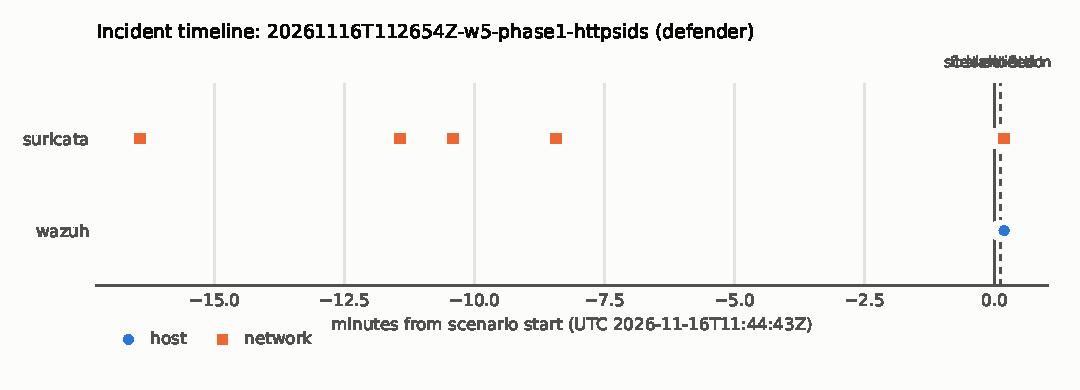
\includegraphics[width=0.98\linewidth]{week5/timeline-20261116T112654Z-w5-phase1-httpsids.pdf}}
      {\framebox[0.9\linewidth]{\rule{0pt}{6cm}timeline (generated)}}
  \end{tikzfigure}
}

\block{7.~Limitations \& conclusion}{
  \begin{itemize}
    \item \textbf{Limitations:} five-node POC; rehearsals on friendly infrastructure;
      containment/recovery not exercised; the graded peer engagement was still pending.
    \item \textbf{Conclusion:} an evidence-first detection pipeline and a
      credential-bounded LLM incident analyst are validated on our own range.
    \item \textbf{Future:} the graded inter-team engagement; wire in the allocated
      A100/H200 model backend; extend the detection set as scenarios demand.
  \end{itemize}
}

\end{columns}

%% ---------------- FULL-WIDTH REPRODUCIBILITY STRIP ----------------
\block{Reproducibility}{
  \begin{center}\small
  Baseline \texttt{main@17d6520} \quad$\cdot$\quad
  images by digest: ACP \texttt{@b1289eab}, Hermes \texttt{@73fbc343},
  \texttt{llama.cpp sha-537c5c0de2f6} (\texttt{qwen2.5-0.5b-instruct}) \quad$\cdot$\quad
  runs \texttt{20261116T100522Z}, \texttt{20261116T112654Z} \quad$\cdot$\quad
  figures via \texttt{project/tools/w5paper.sh} \quad$\cdot$\quad
  repo \texttt{github.com/chpc-tech-eval/purple-team1-scc26}
  \end{center}
}

\end{document}
